\paragraph[QuizziPedia::Front-End::Controllers\\::RegistrationManagementController]{QuizziPedia::Front-End::Controllers::RegistrationManagementController}
\begin{figure} [ht]
	\centering
	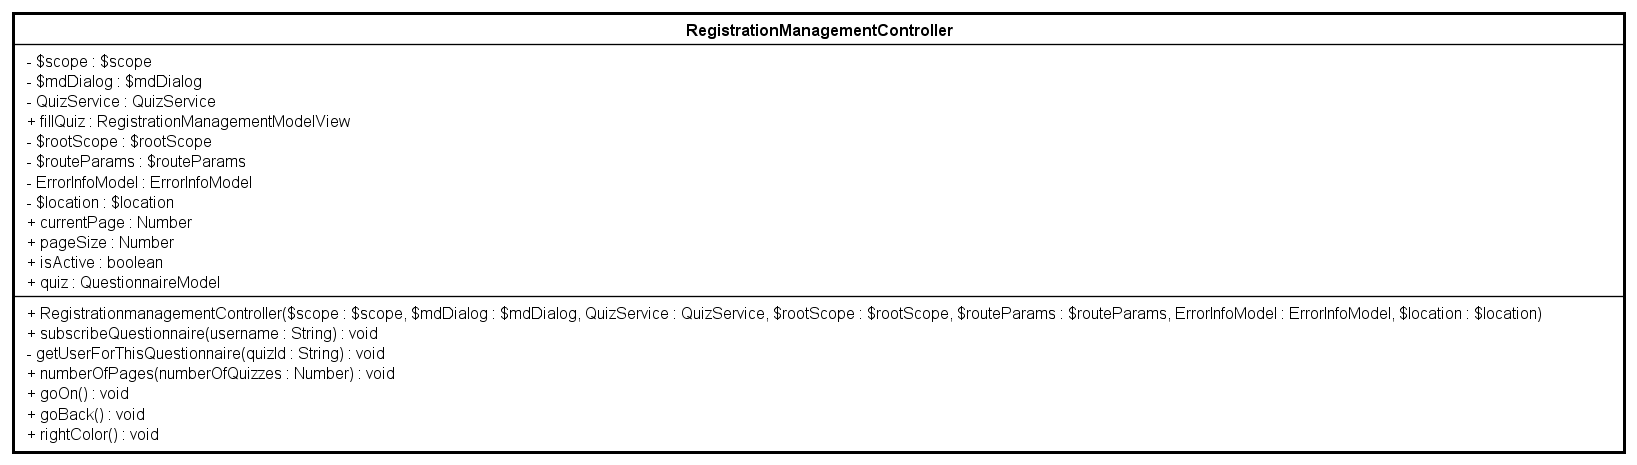
\includegraphics[scale=0.3]{UML/Classi/Front-End/QuizziPedia_Front-end_Controller_RegistrationManagementController.png}
	\caption{QuizziPedia::Front-End::Controllers::RegistrationManagementController}
\end{figure} \FloatBarrier
\begin{itemize}
	\item \textbf{Descrizione}: questa classe permette di gestire le iscrizione degli utenti ai questionari;
	\item \textbf{Utilizzo}: fornisce le funzionalità di iscrizione ad un questionario;
	\item \textbf{Relazione con altre classi}:
	\begin{itemize}
		\item \textbf{IN \texttt{RegistratioManagementModelView}}: classe di tipo \textit{modelview\ped{G}} la cui istanziazione è contenuta all'interno della variabile di ambiente \$scope di \textit{Angular\ped{G}}. All'interno di essa sono presenti le variabili e i metodi necessari per il \textit{Two-Way Data-Binding\ped{G}} tra la \textit{view\ped{G}} \texttt{RegistrationManagementView} e il \textit{controller\ped{G}} \texttt{RegistrationManagementCont-\\roller}; 
		\item \textbf{OUT \texttt{QuizService}}: questa classe permette di ottenere i dati di un quiz tramite delle parole chiave inserite dall'utente nella barra di ricerca.
	\end{itemize}
	\item \textbf{Attributi}:
	\begin{itemize}
		\item \texttt{-} \texttt{\$scope: \$scope} \\
		Campo dati contenente un riferimento all'oggetto \$scope creato da \textit{Angular\ped{G}}, viene utilizzato come mezzo di comunicazione tra il \textit{controller\ped{G}} e la \textit{view\ped{G}}. Contiene gli oggetti che definiscono il \textit{model\ped{G}} dell'applicazione;
		\item \texttt{-} \texttt{\$mdDialog: \$mdDialog} \\
		Campo dati contenente un riferimento al servizio della libreria \textit{Material for Angular\ped{G}} che permette di creare delle componenti a pop-up;
		\item \texttt{-} \texttt{QuizService: QuizService}\\ parametro che permette di ottenere, tramite il \textit{service\ped{G}}, la lista di tutte le domande presenti nel quiz;
		\item \texttt{+} \texttt{fillQuiz: RegistrationManagementModelView} \\
		Oggetto di tipo \texttt{RegistrationManagementModelView}. All'interno di esso sono presenti le variabili e i metodi necessari per il \textit{Two-Way Data-Binding\ped{G}} tra la \textit{view\ped{G}} \texttt{RegistrationManagemenView} e il \textit{controller\ped{G}} \texttt{RegistrationManagemenController};
		\item \rootscopeA;
		\item \routeparamsA;
		\item \errorinfomodelA;
		\item \locationA;
		\item \texttt{+} \texttt{currentPage: Number} \\ Campo dati che indica la pagina corrente per la visualizzazione dei questionari;
		\item \texttt{+} \texttt{pageSize: Number} \\Campo dati che contiene il numero massimo di questionari visualizzabili per pagina;
		\item \texttt{+} \texttt{isActive: Boolean} \\Campo dati che indica se attivo o meno;
		\item \texttt{+} \texttt{quiz: QuestionnaireModel} \\.

	\end{itemize}
	\item \textbf{Metodi}:
	\begin{itemize}
		\item \texttt{+} \texttt{RegistrationmanagementController(\$scope: \$scope, \$mdDialog: \$mdDia-\\log, QuizService: QuizService, \$rootScope: \$rootScope, \$routeParams: \$routeParams, ErrorInfoModel: ErrorInfoModel, \$location: \$location)}: \\Metodo costruttore della classe. \\
			\textbf{Parametri}:
			\begin{itemize}
					\item \texttt{\$scope: \$scope} \\
					Campo dati contenente un riferimento all'oggetto \$scope creato da \textit{Angular\ped{G}}. Viene utilizzato come mezzo di comunicazione tra il \textit{controller\ped{G}} e la \textit{view\ped{G}}. Contiene gli oggetti che definiscono il \textit{viewmodel\ped{G}} e il \textit{model\ped{G}} dell'applicazione;
					\item \texttt{\$mdDialog: \$mdDialog} \\
					Campo dati contenente un riferimento al servizio della libreria \textit{Material for Angu-\\lar\ped{G}} che permette di creare delle componenti a pop-up;
					\item \texttt{QuizService: QuizService}: parametro che permette di ottenere, tramite il \textit{service\ped{G}}, la lista di tutte le domande presenti nel quiz;
					\item \rootscopeP;
					\item \routeparamsP;
					\item \errorinfomodelP;
					\item \locationP. 
			\end{itemize}
		\item \texttt{+} \texttt{subscribeQuestionnaire(username: String): void} \\ Metodo che permette l'iscrizione ad un questionario. Richiama la funzionalità del \texttt{QuizService}. \\
		\textbf{Parametri}:
		\begin{itemize}
			\item \texttt{username: String}: parametro che indica l'utente da iscrivere al questionario.
		\end{itemize}
		
		
		\item \texttt{-} \texttt{getUserForThisQuestionnaire(quizId: String): void} \\ Metodo che permette restituire gli utenti per di un questionario. \\
		\textbf{Parametri}:
		\begin{itemize}
			\item \texttt{quizId: String}: parametro che indica l'id del questionario.
		\end{itemize}
		\item \texttt{+} \texttt{numberOfPages(numberOfQuizzes: Number): void} \\ Metodo che permette di calcolare il numero di pagine da mostrare. \\
		\textbf{Parametri}:
		\begin{itemize}
			\item \texttt{numberOfQuizzes: Number}: parametro che indica il numero di questionari presenti.
		\end{itemize}
		\item \texttt{+} \texttt{goOn(): void} \\ Metodo che permette di andare alla pagina successiva; \\
		\item \texttt{+} \texttt{goBack(): void} \\ Metodo che permette di andare alla pagina precedente; \\
		\item \texttt{+} \texttt{rightColor(): void} \\ Metodo che permette di impostare il giusto colore. \\
		
	\end{itemize}
\end{itemize}

